\documentclass[sigconf]{acmart}

\usepackage{booktabs} % For formal tables

\usepackage{amsmath}
\usepackage{float}
\usepackage{hyperref}
\usepackage{listings}
\usepackage{algorithm}
\usepackage[noend]{algpseudocode}
\usepackage{graphicx}
\usepackage{courier}
\usepackage{float}
\usepackage{color}
\usepackage[margin=10pt,font=small,labelfont=bf,
  labelsep=endash]{caption}
\usepackage{ulem}

\usepackage{syntax} % for writing BNF grammar

\usepackage{forest}
\usepackage{framed}

\usepackage{tikz}
\usetikzlibrary{matrix}
\usetikzlibrary{shapes.multipart}
\usetikzlibrary{patterns}
\usetikzlibrary{positioning,fit,calc}
\usetikzlibrary{decorations.pathmorphing}
\usetikzlibrary{decorations.pathreplacing}
\usetikzlibrary{quotes}
\usetikzlibrary{graphs}
\usetikzlibrary{arrows.meta}
\usetikzlibrary{shapes}
% \usetikzlibrary{graphs,graphdrawing}
% \usegdlibrary{layered}
% \usetikzlibrary{graphdrawing,graphs,calc}
% \usegdlibrary{layered}

\usepackage{smartdiagram}

% \usetikzlibrary{external}
% \tikzexternalize % activate!
% \tikzset{external/force remake}

%% To generate figure, uncomment above three lines, and execute:
%% pdflatex -shell-escape helium.tex

\usepackage{csvsimple}
\usepackage{multirow}


\lstset{basicstyle=\footnotesize\ttfamily,breaklines=true}
% \lstset{frame=b}
\lstset{float,floatplacement=H,captionpos=b}
% \lstset{numbers=left}
\lstset{language=C}
\lstset{showstringspaces=false}
\lstset{breakindent=10pt}
% \lstset{framextopmargin=10pt}
% \lstset{framextopmargin=50pt,frame=t}
% \lstset{float=htb,language=C,frame=single, basicstyle=\small, stringstyle=\ttfamily}
% \lstset{escapeinside={(*@}{@*)}}
% \usepackage{xcolor}
\lstdefinestyle{base}{
  language=C,
  emptylines=1,
  breaklines=true,
  aboveskip=0em,
  belowskip=0em,
  % float,
  % floatplacement=H,
  basicstyle=\footnotesize\ttfamily\color{black},
  moredelim=**[is][\color{blue}]{@}{@},
  moredelim=**[is][\color{purple}]{~1}{~1},
  moredelim=**[is][\color{brown}]{~2}{~2},
  moredelim=**[is][\color{gray}]{~3}{~3},
  moredelim=**[is][\color{orange}]{~4}{~4},
  moredelim=**[is][\color{violet}]{~5}{~5},
}
\lstdefinestyle{graycode} {
  language=C,
  emptylines=1,
  breaklines=true,
  basicstyle=\footnotesize\ttfamily\color{gray!50},
  moredelim=**[is][\color{blue}]{@}{@},
}
\lstset{style=base}


\title{How to compute}
% \lstset{numbers=left}
\begin{document}

\begin{figure*}
  \centering
  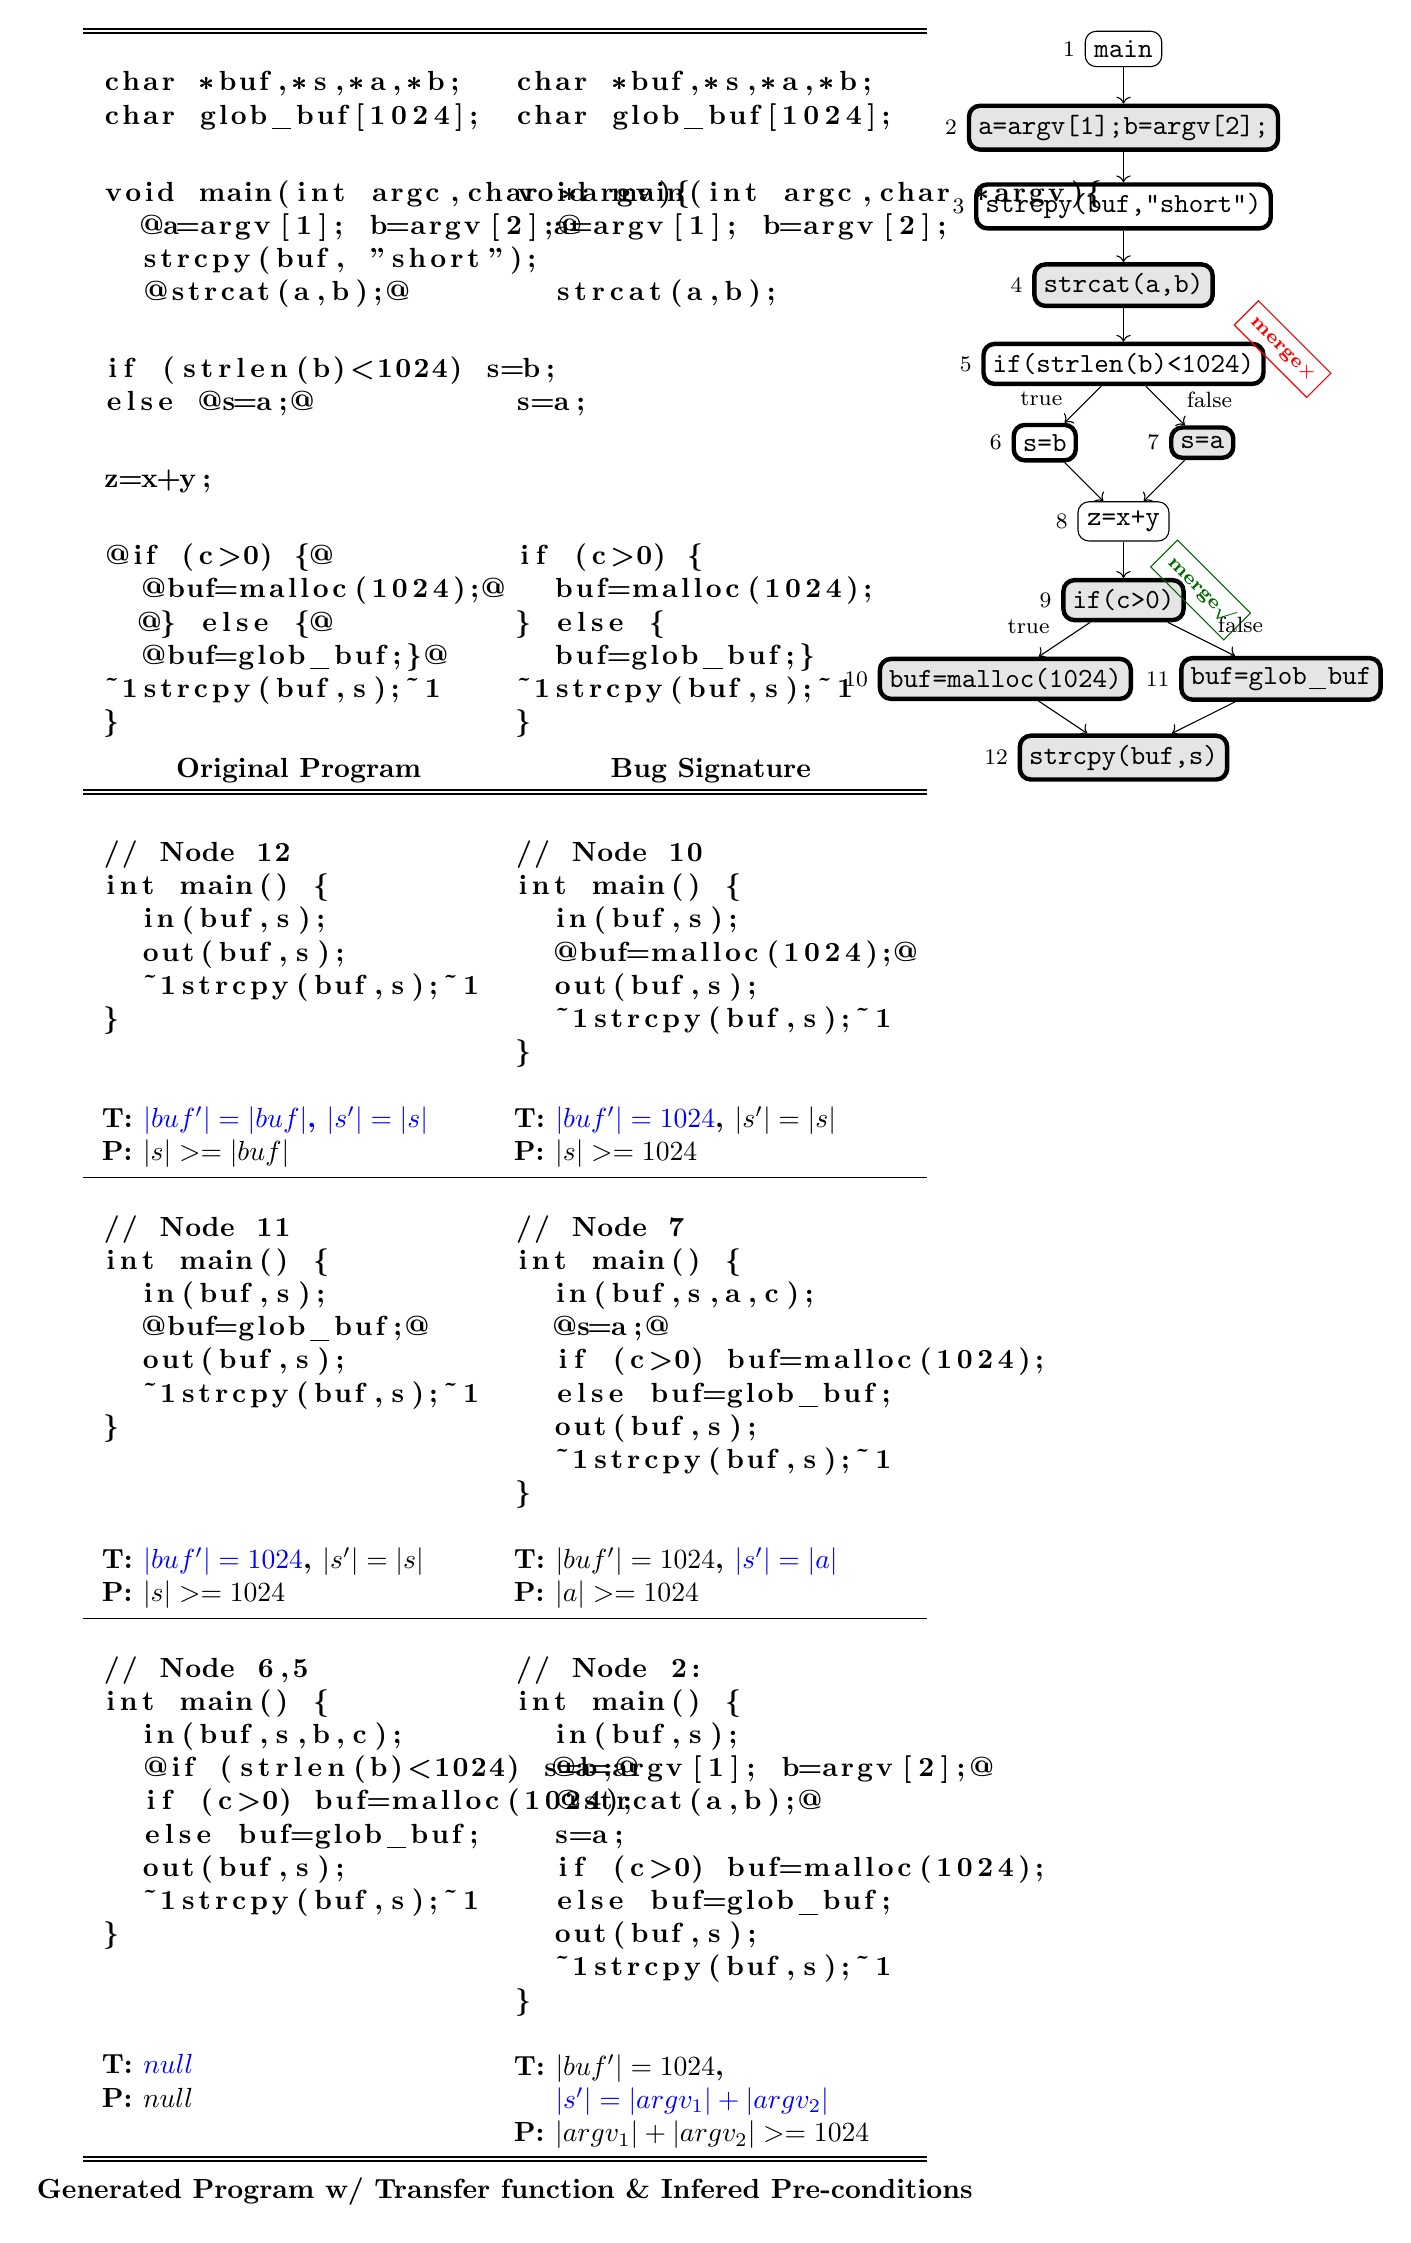
\begin{tikzpicture}[every label quotes/.style={left, font=\footnotesize},
      cfg/.style={draw,rectangle,rounded corners},
      tf/.style={text=\scriptsize},
      trans/.style={align=center,draw,rounded corners,rectangle
        split,rectangle split parts=2,draw,dashed,fill=gray!10!white,minimum width=5cm,font=\scriptsize\bfseries},
      bench/.style={draw,fill=gray!20!white},
      slice/.style={draw,ultra thick},
      merge label/.style={red,font=\scriptsize\bfseries,draw,rotate=-45,label position=40},
      every label/.style={font=\normalsize},
      num/.style={draw,circle},
      label position={0},
      font=\bfseries,
      ]

    \graph[grow down, branch right,
      nodes={draw,rectangle,rounded corners},
      ->
      % draw,
      ] {main/\texttt{main}["1"]
      -> "\texttt{a=argv[1];b=argv[2];}"[bench, slice, "2"]
      -> strcpy/"\texttt{strcpy(buf,"short")}"[slice,"3"]
      -> "\texttt{strcat(a,b)}"[bench,slice,"4"]
      -> "\texttt{if(strlen(b)<1024)}"[slice,"5",
        label={[merge label,shift={(6mm,9mm)}]merge$\times$}]
      -> [edge quotes={auto,pos=0.8,font=\footnotesize}]
      {
        "\texttt{s=b}"[slice,shift={(-1,0)}, > "true"',"6"],
        "\texttt{s=a}"[bench,slice,> "false","7"]
      }
      -> "\texttt{z=x+y}"["8"]
      -> c8/"\texttt{if(c>0)}"[bench,slice,"9",
        label={[merge label,shift={(-1mm,1mm)},green!40!black]merge$\surd$}]
      -> [edge quotes={auto, pos=0.6,font=\footnotesize}]
      {
        "\texttt{buf=malloc(1024)}"[bench,slice,shift={(-1.5,0)},> "true"',"10"],
        "\texttt{buf=glob_buf}"[shift={(1,0)},bench,slice,> "false","11"]}
      -> poi/"\texttt{strcpy(buf,s)}"[bench,slice,"12"]
    };
    
    \matrix (full) [
      left=2.5cm of main.north,
      matrix anchor=north east,
      every node/.style={
        % draw,
        inner ysep=0,
        text width=5cm,
        % inner xsep=10pt,
      },
      % column sep=3pt,
      anchor=north west,
      every label quotes/.style={below,font=\footnotesize},
      % align=center,
      % column sep=10pt,
      % draw
      ] {

      %% I'm going to split the code into parts

      \node {
\begin{lstlisting}
char *buf,*s,*a,*b;
char glob_buf[1024];
\end{lstlisting}        
      };&
      \node {
\begin{lstlisting}
char *buf,*s,*a,*b;
char glob_buf[1024];
\end{lstlisting}
      };\\
      \node {
\begin{lstlisting}
void main(int argc,char *argv){
  @a=argv[1]; b=argv[2];@
  strcpy(buf, "short");
  @strcat(a,b);@
\end{lstlisting}
      };&
      \node {
\begin{lstlisting}
void main(int argc,char *argv){
  a=argv[1]; b=argv[2];

  strcat(a,b);
\end{lstlisting}
      };\\
      \node {
\begin{lstlisting}
if (strlen(b)<1024) s=b;
else @s=a;@
\end{lstlisting}
      };&
      \node {
\begin{lstlisting}

s=a;
\end{lstlisting}
      };\\
      \node {
\begin{lstlisting}
z=x+y;
\end{lstlisting}
      };&
      \node {
\begin{lstlisting}
\end{lstlisting}
      };\\
      \node {
\begin{lstlisting}
@if (c>0) {@
  @buf=malloc(1024);@
  @} else {@
  @buf=glob_buf;}@
~1strcpy(buf,s);~1
}
\end{lstlisting}
      };&
      \node {
\begin{lstlisting}
if (c>0) {
  buf=malloc(1024);
} else {
  buf=glob_buf;}
~1strcpy(buf,s);~1
}
\end{lstlisting}
      };\\
      \node [align=center] {
        Original Program
      };&
      \node [align=center] {
        Bug Signature
      };\\
    };
    % \draw (0,0) grid (10,10);

    \matrix (gen) [
      matrix anchor=north west,
      "Generated Program w/ Transfer function \& Infered Pre-conditions"
      {below, font=\normalsize\bf},
      below=0pt of full.south west,
      % draw,
      % matrix of nodes,
      every node/.style={
        text width=5cm,
        % inner sep=0,
        align=left,
        % draw
      }
      ] {
      \node {
\begin{lstlisting}
// Node 12
int main() {
  in(buf,s);
  out(buf,s);
  ~1strcpy(buf,s);~1
}
\end{lstlisting}        
      };&
      \node {
\begin{lstlisting}
// Node 10
int main() {
  in(buf,s);
  @buf=malloc(1024);@
  out(buf,s);
  ~1strcpy(buf,s);~1
}
\end{lstlisting}        
      };\\
      \node  (t1) {
        T: {\color{blue}$|buf'|=|buf|$, $|s'|=|s|$}\\
        P: $|s| >= |buf|$
      };&
      \node {
        T: {\color{blue}$|buf'|=1024$}, $|s'|=|s|$\\
        P: $|s| >= 1024$
      };\\
      \node {
\begin{lstlisting}
// Node 11
int main() {
  in(buf,s);
  @buf=glob_buf;@
  out(buf,s);
  ~1strcpy(buf,s);~1
}
\end{lstlisting}        
      };&
      \node {
\begin{lstlisting}
// Node 7
int main() {
  in(buf,s,a,c);
  @s=a;@
  if (c>0) buf=malloc(1024);
  else buf=glob_buf;
  out(buf,s);
  ~1strcpy(buf,s);~1
}
\end{lstlisting}        
      };\\
      \node (t2) {
        T: {\color{blue}$|buf'|=1024$}, $|s'|=|s|$\\
        P: $|s| >= 1024$
      };&
      \node {
        T: $|buf'|=1024$, {\color{blue}$|s'|=|a|$}\\
        P: $|a| >= 1024$
      };\\
      \node {
\begin{lstlisting}
// Node 6,5
int main() {
  in(buf,s,b,c);
  @if (strlen(b)<1024) s=b;@
  if (c>0) buf=malloc(1024);
  else buf=glob_buf;
  out(buf,s);
  ~1strcpy(buf,s);~1
}
\end{lstlisting}
      };&
      \node {
\begin{lstlisting}
// Node 2:
int main() {
  in(buf,s);
  @a=argv[1]; b=argv[2];@
  @strcat(a,b);@
  s=a;
  if (c>0) buf=malloc(1024);
  else buf=glob_buf;
  out(buf,s);
  ~1strcpy(buf,s);~1
}
\end{lstlisting}
      };\\
      \node {
        T: {\color{blue}$null$}\\
        P: $null$
      };&
      \node (t3) {
        T: $|buf'|=1024$,\\
        {\color{white}T:} {\color{blue}$|s'|=|argv_1|+|argv_2|$}\\
        P: $|argv_1|+|argv_2|>=1024$
      };\\
    };

    % \draw (gen-1-1) -- (gen-1-2);
    \draw [double, thick] (full.north west) -- (full.north east);
    \draw [double, thick] (full.south west) -- (full.south east);
    \draw (t1.south -| gen.west) -- (t1.south -| gen.east);
    \draw (t2.south -| gen.west) -- (t2.south -| gen.east);
    \draw [double, thick] (t3.south -| gen.west) -- (t3.south -| gen.east);
    
  \end{tikzpicture}
\end{figure*}

\end{document}
